%\newcommand{\CH}[1]{\textbf{\textcolor{green}{CH - #1}}}
\subsubsection{\theoryC{$Z'$ discrimination at HE-LHC in case of an evidence/discovery after HL-LHC}}
\contributors{C. Helsens, D. Jamin, M. L. Mangano, T. Rizzo, M. Selvaggi}
%{\bf Authors: C. Helsens$^1$, D. Jamin$^2$, M. L. Mangano$^3$, T. Rizzo$^4$, M. Selvaggi$^1$}\\
%\newline
%$^1$CERN EP-Departement, CH-1211 Geneva 23, Switzerland email: {\tt B.C. clement.helsens@cern.ch}\\
%$^2$Academia Sinica, Institute of  Physics, Taipei, Taiwan\\
%$^3$CERN TH-Departement, CH-1211 Geneva 23, Switzerland\\
%$^4$SLAC National Accelerator Laboratory 2575 Sand Hill Rd., Menlo Park, CA, 94025 USA\\

\newcommand*{\sqrtslhc}{\ensuremath{\sqrt{s}=\text{14 TeV}}}
\newcommand*{\sqrtshelhc}{\ensuremath{\sqrt{s}=\text{27 TeV}}}
\renewcommand*{\intlumihelhc}{\ensuremath{\mathcal{L}=15\text{ ab}^{-1}}}
\newcommand*{\intlumihllhc}{\ensuremath{\mathcal{L}=3\text{ ab}^{-1}}}


%%%%%%%%%%%%%%%%%%%%%%%%%%%%%%%%%%%%%%%%%%%%%%%%%%%%%
%\subsection{Context of the study}
\paragraph*{Context of the study}
It is still legitimate to assume that a heavy resonance could be seen at the end of HL-HLC. If that is the case a new collider with higher energy
in the \com is needed to study its properties as too few events will be available at \sqrtslhc. In this section we present the discrimination potential between six $Z'$ models of a High Energy LHC (HE-LHC) with an assumed \com energy of 27~TeV and an integrated luminosity of \intlumihelhc. Under the assumption that these $Z'$'s decay only to SM particles, we show that there are sufficient observables to perform this model differentiation in most cases.

%%%%%%%%%%%%%%%%%%%%%%%%%%%%%%%%%%%%%%%%%%%%%%%%%%%%%
%\subsection{Bounds from HL-LHC}
\paragraph*{Bounds from HL-LHC}
As a starting point it is needed to estimate what are, for $\sqrt s=14$ TeV, the typical exclusion/discovery reaches for standard reference $Z'$ models assuming \intlumihllhc\ employing only the $e^+e^-$ and $\mu^+\mu^-$ channels. To address this and the other questions below we will use the same set of $Z'$ models as employed
in Ref.~\cite{Rizzo:2014xma} and mostly in Ref.~\cite{Han:2013mra}, both of which we will refer to frequently. We employ the MMHT2014 NNLO PDF set~\cite{Harland-Lang:2014zoa}
throughout with an appropriate constant $K$-factor (=1.27) to account for higher order QCD corrections. The production cross section times leptonic branching fraction is shown in Figure~\ref{fig:pheno:toy} (left) for these models at \sqrtslhc\ in the narrow width approximation (NWA). It has been and will be assumed here that these $Z'$ states only decay to SM particles.


\begin{figure}[htbp]
  \centering
    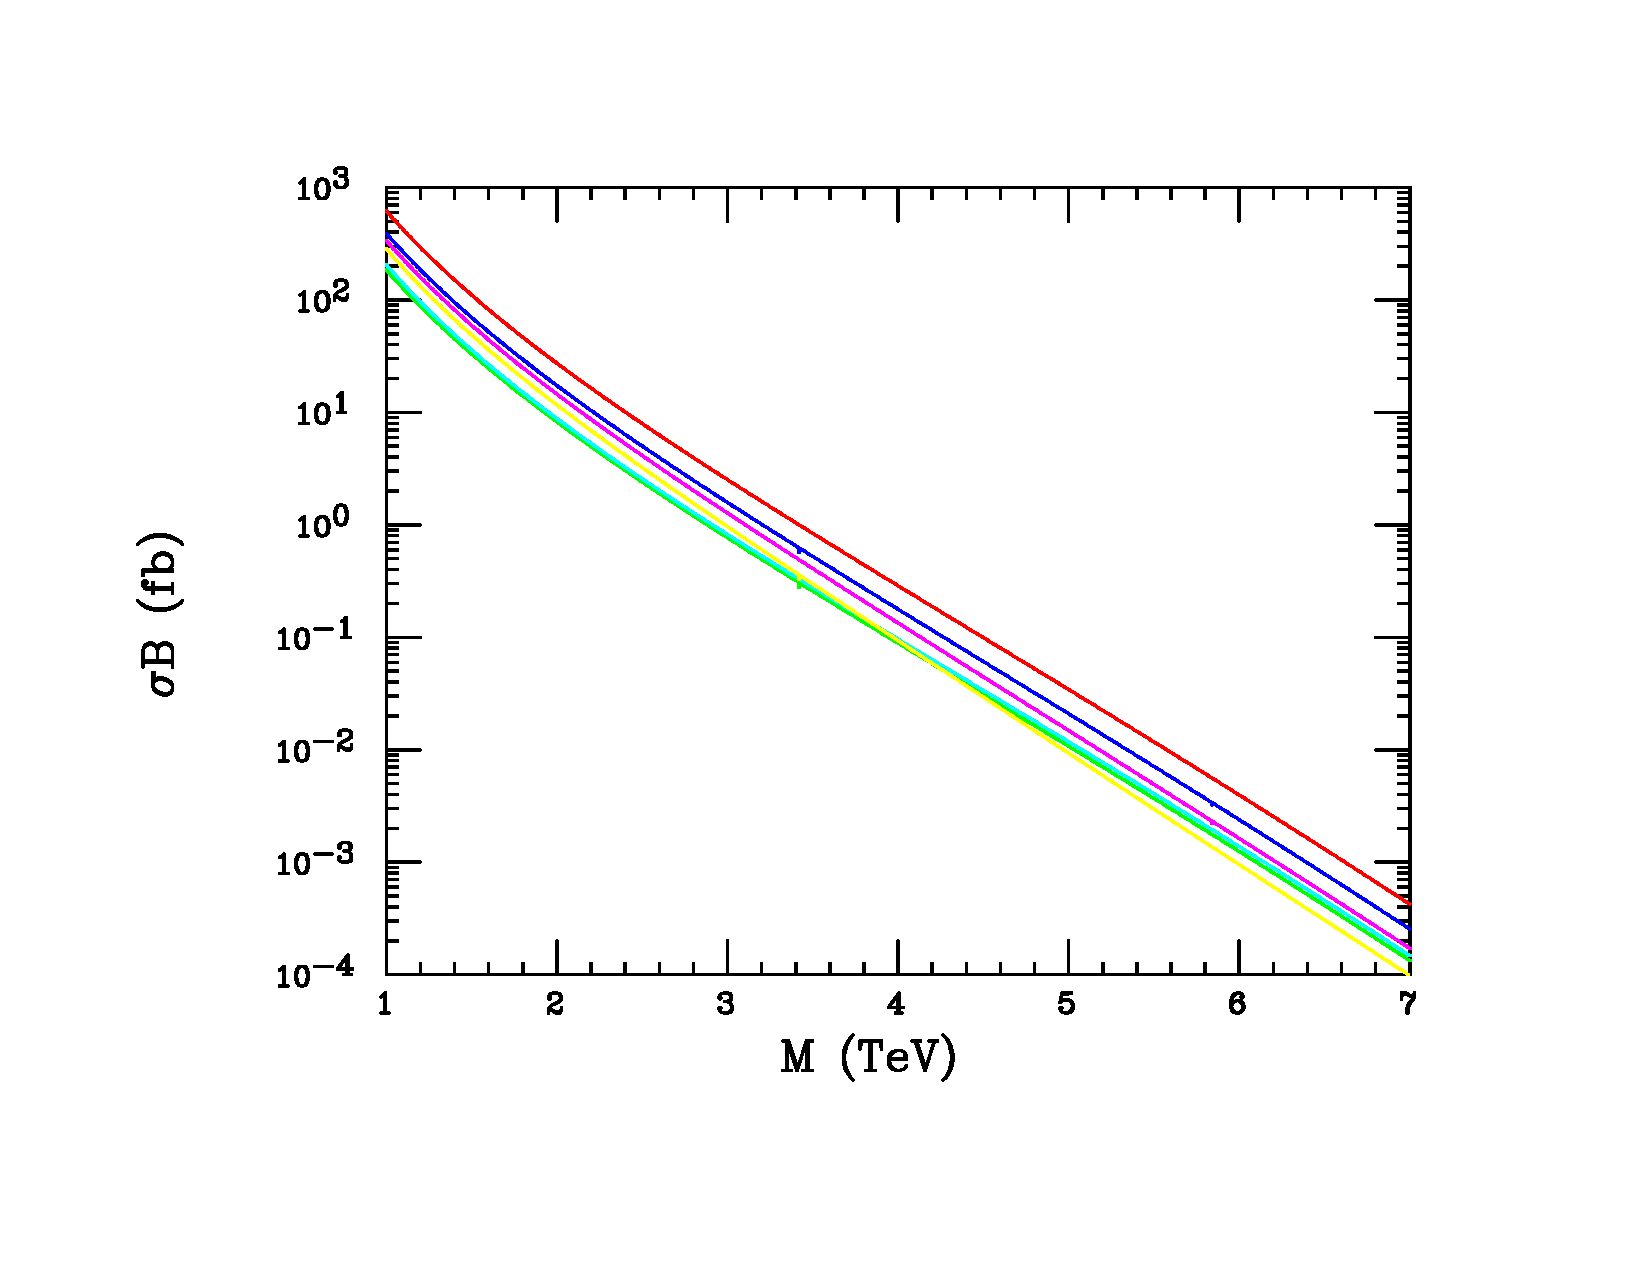
\includegraphics[trim={2cm 2cm 2cm 2cm},clip,width=0.45\columnwidth]{\main/section7OtherSignatures/img/zp14tev-ref.pdf}
    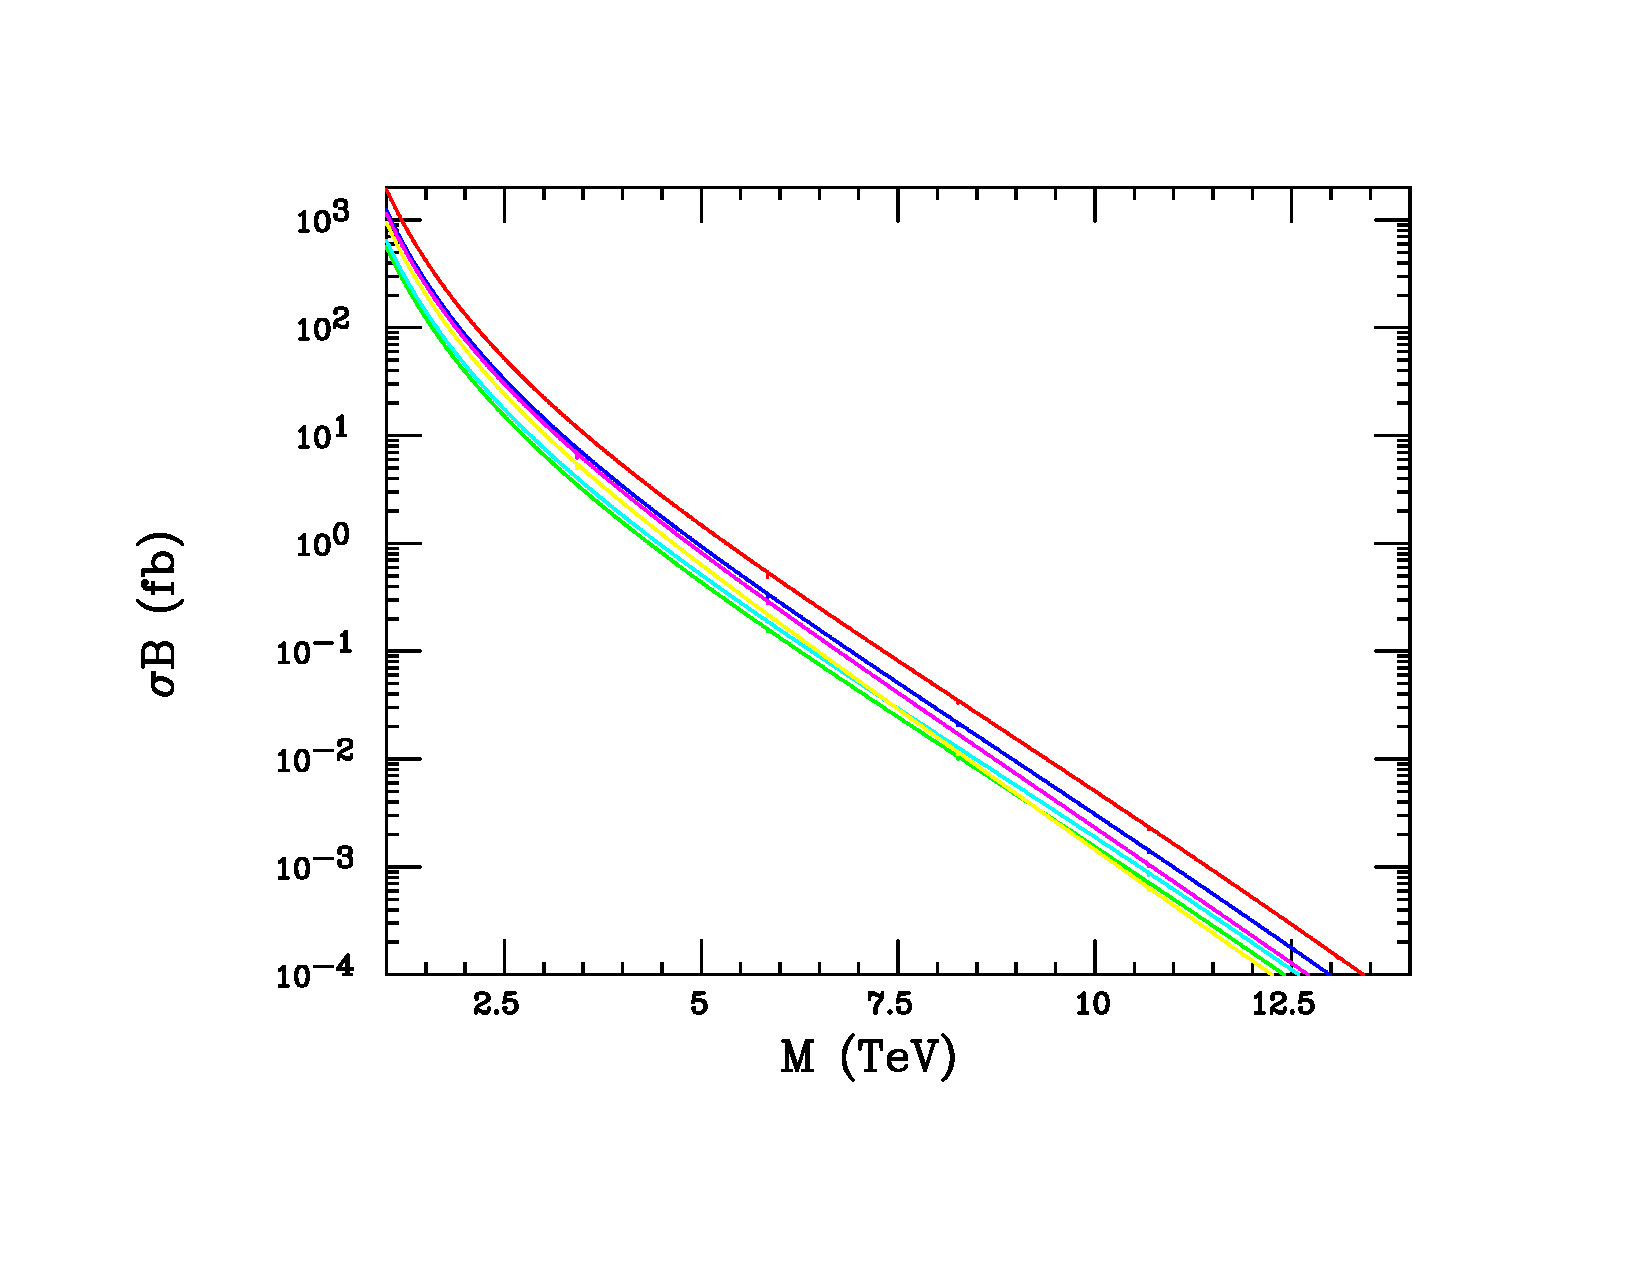
\includegraphics[trim={2cm 2cm 2cm 2cm},clip,width=0.45\columnwidth]{\main/section7OtherSignatures/img/zp27tev-ref.pdf}
    \caption{Left: $\sigma B_l$ in the NWA for the $Z'$ production at the $\sqrt s=14$ TeV LHC as functions of the $Z'$ mass: SSM(red), LRM (blue), $\psi$(green), $\chi$(magenta),
$\eta$(cyan), I(yellow). (Right) $\sigma B_l$ of $Z'$ in models described in (left) at $\sqrt s=27$ TeV.}
\label{fig:pheno:toy}
\end{figure}

Using the present ATLAS and CMS results at 13 TeV,~\cite{Aaboud:2017buh} and~\cite{Sirunyan:2018exx}, it is straightforward to estimate by extrapolation the
exclusion reach at \sqrtslhc\ using the combined $ee+\mu\mu$ final states. This is given in the first column of Table~\ref{tab:pheno:spec}. For discovery, only the $ee$ channel is used due to poor $\mu\mu$-pair invariant mass resolution near $M_{Z'}=6$ TeV. Estimates of the $3\sigma$ evidence and $5\sigma$
discovery limits are also given in Table~\ref{tab:pheno:spec}. Based on these results, we will assume in our study below that we are dealing with a $Z'$ of mass 6 TeV. Figure~\ref{fig:pheno:toy} (right) shows the NWA cross sections for the same set of models but now at \sqrtshelhc\ with \intlumihelhc. We note that very large statistical samples will be available for the case of $M_{Z'}=6$ TeV
for each dilepton channel.

%
\begin{table}
\centering
\begin{tabular}{|l|c|c|c|} \hline\hline
  Model &   95$\%$ \cl  &  $3\sigma$  & $5\sigma$   \\
\hline
SSM    &     6.62     &  6.09    &  5.62     \\
LRM    &   6.39     & 5.85     & 5.39  \\
$\psi$    &  6.10   & 5.55   & 5.07  \\
$\chi$   &  6.22    & 5.68    & 5.26   \\
$\eta$   &  6.15     &  5.59  &  5.16   \\
~I        & 5.98   &  5.45   &  5.05  \\
\hline\hline
\end{tabular}
\caption{ Mass reach for several $Z'$ models at \sqrtslhc\ with \intlumihllhc. }
\label{tab:pheno:spec}
\end{table}
%
\paragraph*{Definition of the discriminating variables}
\label{par:vardef}

The various $Z'$ models can be disentangled with the help of 3 inclusive observables: the production cross section times leptonic branching fraction $\sigma B_l$, the forward-backward asymmetry $A_{FB}$ and the rapidity ratio $r_y$. The variable $A_{FB}$ can be seen as an estimate of the charge asymmetry
\begin{equation}
A_{FB} = A_C =  \frac{\sigma(\Delta|y| > 0) - \sigma(\Delta|y| < 0)}{\sigma(\Delta|y| > 0) + \sigma(\Delta|y| < 0)},
\end{equation}
where $\Delta|y| = |y_l| - |y_{\bar{l}}|$. It has been checked that this definition is equivalent to defining
\begin{equation}
A_{FB} = \frac{\sigma_F - \sigma_B}{\sigma_F + \sigma_B},
\end{equation}
with $\sigma_F = \sigma (cos\theta^{*}_{cs})>0$ and $\sigma_B = \sigma (cos\theta^{*}_{cs})<0$ where $\theta^*_{cs}$ is the Collins-Soper frame angle. The variable $r_y$ is defined as the ratio of central over forward events:
\begin{equation}
r_y = \frac{\sigma(|y_{Z'}| < y_1)}{\sigma(y_1 < |y_{Z'}| <y_2)},
\end{equation}
where $y_1=0.5$ and $y_2=2.5$.

%%%%%%%%%%%%%%%%%%%%%%%%%%%%%%%%%%%%%%%%%%%%%%%%%%%%%
\paragraph*{Model discrimination}

The model discrimination presented in this section has been performed assuming the HE-LHC detector parametrisation~\cite{hlhelhc_web} in \delphes~\cite{deFavereau:2013fsa}. In such a detector, muons at $\eta \approx 0$ are assumed to be reconstructed with a resolution $\sigma(p)/p \approx 7\%$ for $\pt~=~3 $~TeV.

\subparagraph*{Leptonic final states}
\label{par:lepana}

The potential for discriminating various $Z'$ models is first investigated using the leptonic $ee$ and $\mu\mu$ final states only. The signal samples for the 6 models and the Drell-Yan backgrounds have been generated with \pythia~8.230~\cite{Sjostrand:2014zea} including the interference between the signal and background. The $Z'$ decays assume lepton flavour universality. For a description of the event selection and a discussion of the discovery potential in leptonic final states for the list of $Z'$ models being discussed here, the reader should refer to Section~\cite{subsubsec:hr_lep}. We simply point out here that with \intlumihelhc\,, all $Z'$ models with $m_{Z'}~\lesssim~10$~TeV can be excluded at \sqrtshelhc.

Figure~\ref{fig:ana:res} (left) shows the correlated predictions for the $A_{FB}$ and the rapidity ratio $r_y$ observables defined previously for these six models given the above assumptions. Although the interference with the SM background was included in the simulation, its effect is unimportant due to the narrowness of the mass window around the resonance that was employed. Furthermore, the influence of the background uncertainty on the results has been found to have little to no impact on the model discrimination potential. Therefore the displayed errors on $A_{FB}$ and $r_y$ are of statistical origin only. The results show that apart from a possible near degeneracy in models $\psi$ and $\eta$, a reasonable $Z'$ model separation can indeed be achieved.

Using a profile likelihood technique, the signal strength $\mu$, or equivalently, $\sigma B_l$, can be fitted together with its corresponding error using the the di-lepton invariant mass shape. The quantity $\sigma B_l$ and its total estimated uncertainty is shown in Figure~\ref{fig:ana:res} (center) as a function of the integrated luminosity. The $\sigma B_l$ measurement seems to be able to resolve the degeneracy between the $\psi$ and $\eta$ models with \intlumihelhc. It should be noted however that since the cross-section can easily be modified by an overall rescaling of the couplings, further handles will be needed for a convincing discrimination.
\rt{in plot right FCC Simulation -> HE-LHC simulation. Plot style can also be improved, line instead of boxes in legends. Increase line thickness in for better visibility.}

\begin{figure}[!htb]
  \centering
   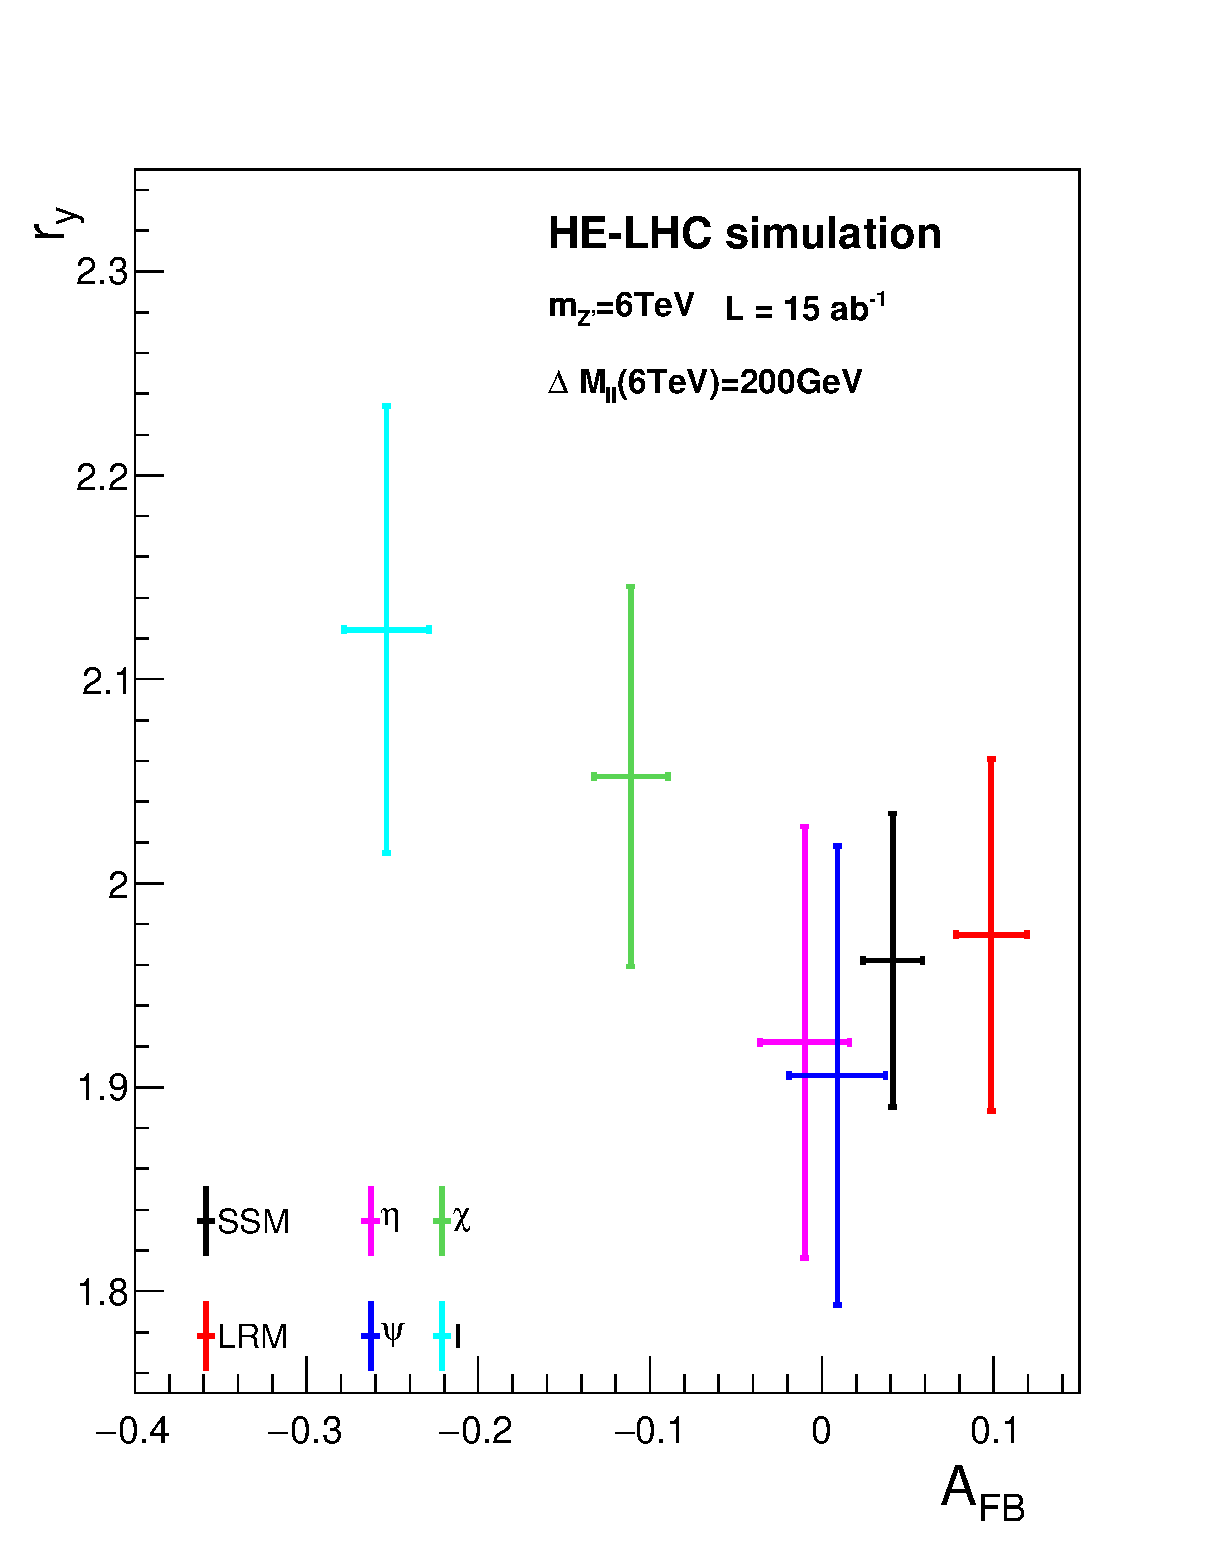
\includegraphics[width=0.30\columnwidth]{\main/section7OtherSignatures/img/ry_afb_200GeV_eta2p5_interf.eps}
   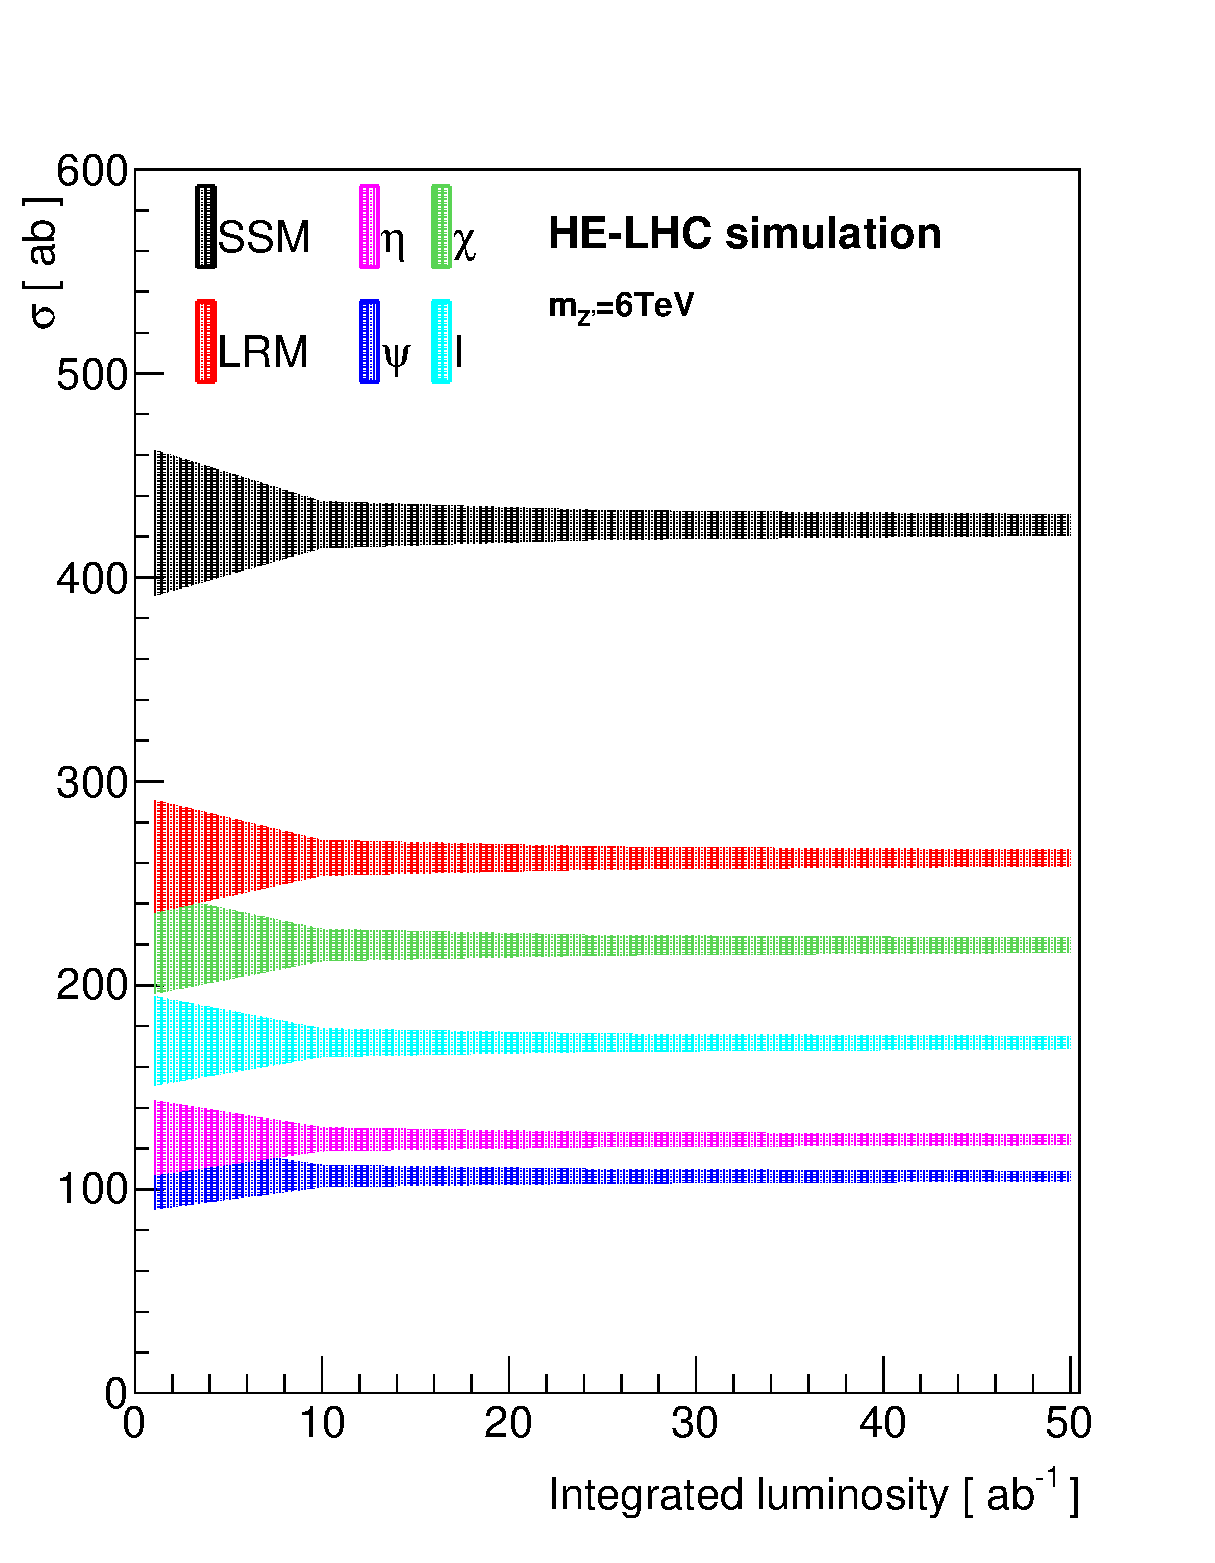
\includegraphics[width=0.30\columnwidth]{\main/section7OtherSignatures/img/sigma_vs_lumi.eps}
   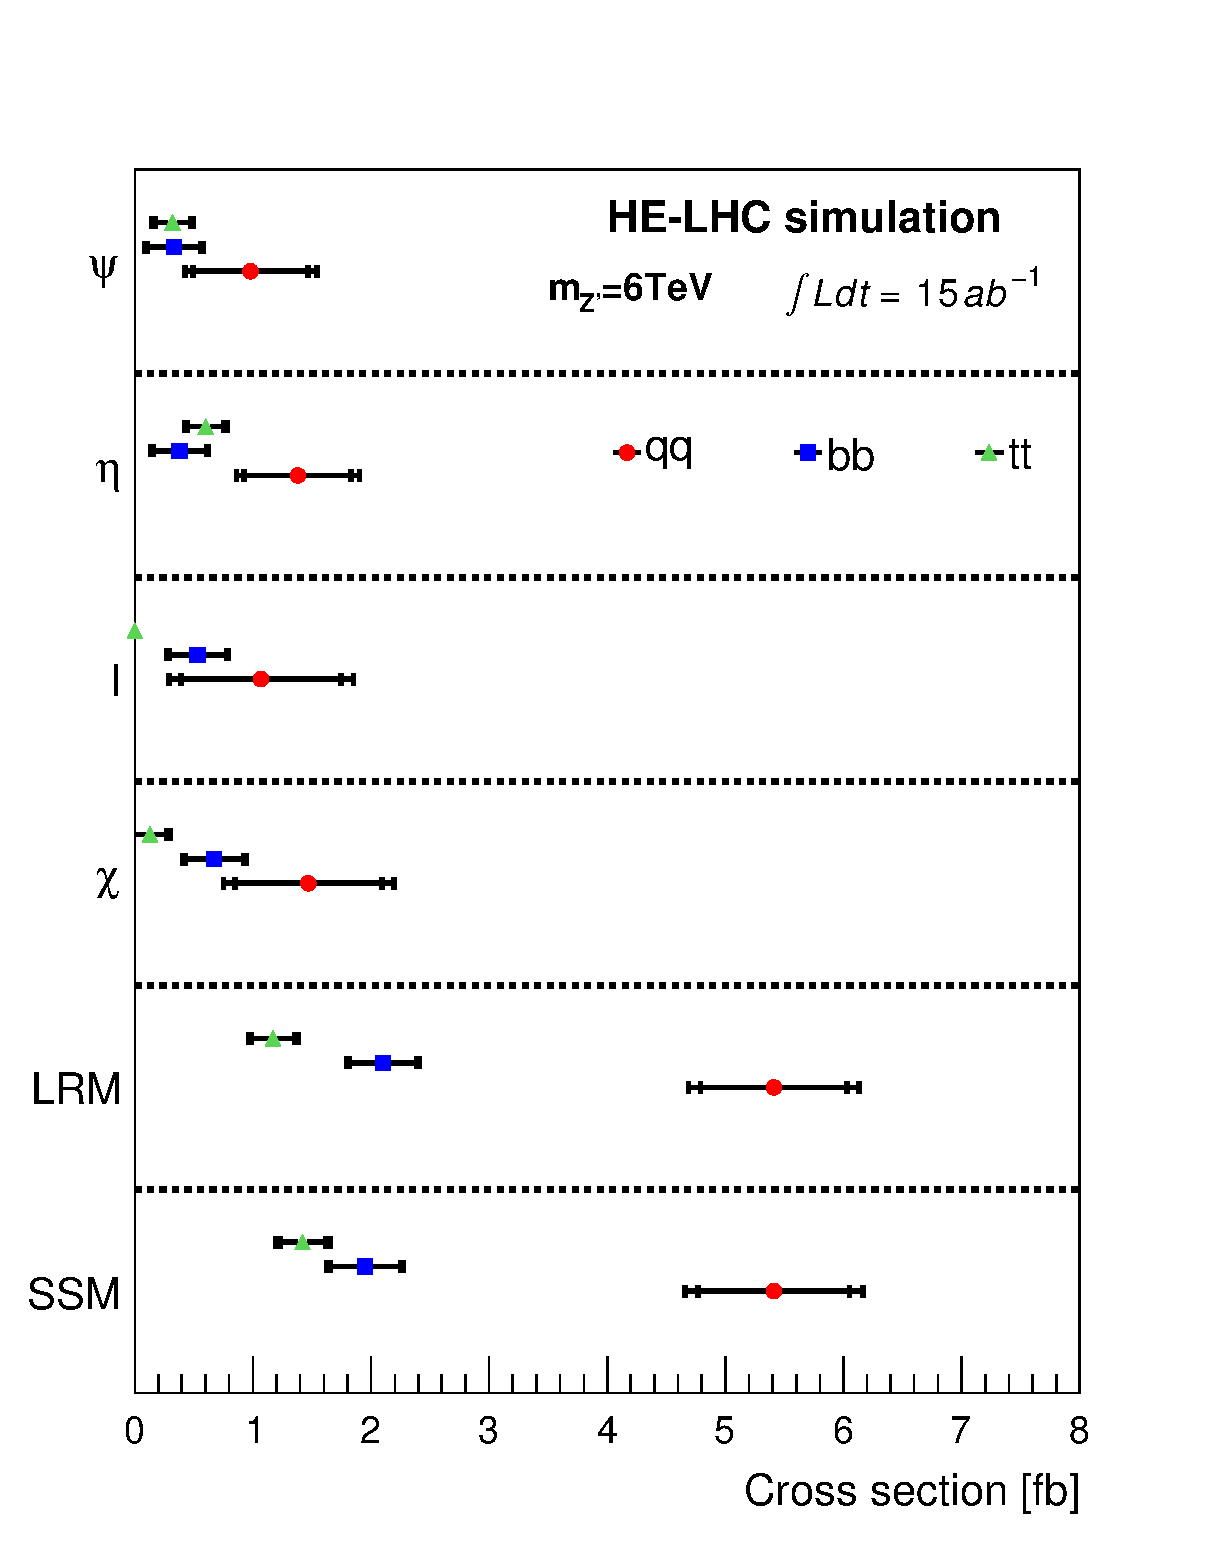
\includegraphics[width=0.30\columnwidth]{\main/section7OtherSignatures/img/Zp_branching_6TeV_15ab.eps}
  \caption{Left: Scatter plot of $r_y$ versus $A_{FB}$ with 200~GeV and mass window. The full interference is included. Center: Fitted signal cross-section together with its corresponding error versus integrated luminosity. Right: Fitted cross-section of the three hadronic analyses. Statistical and full uncertainties are shown on each point.}
  \label{fig:ana:res}
\end{figure}

%%%%%%%%%%%%%%%%%%%%%%%%%%%%%%%%%%%%%%%%%%%%%%%%%%%%%
%\subsubsection{Hadronic analysis}
\subparagraph*{Hadronic final states}
\label{par:hadana}

Model discrimination can be improved by including an analysis involving three $Z'$ addition hadronic final states: $t\bar{t}$, $b\bar{b}$ and $q\bar{q}$, where $q=u,d,c,s$. The sample production and event selection for the $t\bar{t}$, $q\bar{q}$ final states has been described to some extent in Section~\cite{subsubsec:hr_had}. We simply remind the reader that the analysis involves requiring the presence of two central high $\pt$ jets. In order to ensure complete orthogonality between the various final states, jets are required to be tagged as follows. In the $Z' \rightarrow t\bar{t}$ analysis both jets should be \emph{top-tagged}. For the $Z' \rightarrow b\bar{b}$ final state both jets are required to be \emph{b-tagged} and we veto events containing at least one top-tagged jet. Finally, in the $Z' \rightarrow q\bar{q}$ analysis, we veto events that contain at least one b-tagged or top-tagged jet.

Figure~\ref{fig:ana:res} (right) summarises the discrimination potential in terms of fitted cross-section of the different models considering the three aforementionned hadronic decays, $t\bar{t}$,  $b\bar{b}$ and $q\bar{q}$. An good overall discrimination among the various models can be achieved using all possible final states. For example, the SSM and $\psi$ models, which have very close predictions for $r_y$ and $A_{FB}$, have measurably different fractions of $t\bar{t}$ or $b\bar{b}$ final states. We note however that the degeneracy between $\eta$ and $\psi$ can only be partially resolved resolved at $\approx~1~\sigma$ by exploiting the difference in $t\bar{t}$ yield.

\paragraph*{Conclusion}
In this section we studied the discrimination potential of six $Z'$ models at High Energy LHC (HE-LHC) with an assumed \com energy of 27~TeV and an integrated luminosity of \intlumihelhc. The exercise has been performed assuming the evidence of an excess observed at \sqrtslhc\ at a mass $m_{Z'}\approx~6$~TeV. Overall it was found that it is possible to distinguish among most models. Finally, it should be noted that further studies, perhaps employing 3-body decay modes or associated Z' production will be clearly in case of discovery to further characterize the resonance properties. 
